% MARGE User Manual
%
% Please note this document will be automatically compiled and hosted online
% after each commit to master. Because of this, renaming or moving the
% document should be done carefully. To see the compiled document, go to
% https://exosports.github.io/MARGE/doc/MARGE_User_Manual.html

\documentclass[letterpaper, 12pt]{article}
\textwidth=6.5in
\textheight=9.5in
\topmargin=-0.75in
\oddsidemargin=0.0in
\evensidemargin=0.0in

\usepackage{graphicx}
\usepackage{enumitem}
\usepackage{amssymb, amsmath}
\usepackage{xcolor}
\usepackage{listings}

\usepackage{times}
\usepackage{natbib}
\usepackage{etoolbox}
\usepackage{astjnlabbrev-jh}
\usepackage{bibentry}
\usepackage{ifthen}
\usepackage{epsfig}

\usepackage{commath}
\usepackage{rotating}

\usepackage{dirtree}
\usepackage{changepage}
\usepackage{alltt}

%\usepackage[T1]{fontenc}
%\usepackage[scaled]{beramono}
%\usepackage[utf8]{inputenc}
%\renewcommand*\familydefault{\ttdefault}

% \lstset{
% language=Python,
% showstringspaces=false,
% formfeed=\newpage,
% tabsize=4,
% commentstyle=\itshape,
% basicstyle=\ttfamily,
% morekeywords={models, lambda, forms}
% }
 
% \newcommand{\code}[2]{
% \hrulefill
% \subsection*{#1}
% \lstinputlisting{#2}
% \vspace{2em}
% }

% Default fixed font does not support bold face
\DeclareFixedFont{\ttb}{T1}{txtt}{bx}{n}{10} % for bold
\DeclareFixedFont{\ttm}{T1}{txtt}{m}{n}{10}  % for normal
% twelve-sized ttm:
\DeclareFixedFont{\tttb}{T1}{txtt}{bx}{n}{12}  % for bold
\DeclareFixedFont{\tttm}{T1}{txtt}{m} {n}{12}  % for normal

\DeclareFixedFont{\ttnm}{T1}{txtt}{m}{n}{9.8}  % for normal

% Custom colors
\usepackage{color}
\definecolor{deepblue}  {rgb}{0.0, 0.0, 0.5}
\definecolor{deepred}   {rgb}{0.8, 0.0, 0.0}
\definecolor{deepgreen} {rgb}{0.0, 0.5, 0.0}
\definecolor{commentc}  {rgb}{0.5, 0.5, 0.5}
\definecolor{DodgerBlue}{rgb}{0.1, 0.6, 1.0}

% Python style for highlighting
\newcommand\pythonstyle{\lstset{
language=Python,
basicstyle = \ttm,
morekeywords = {self, as, assert, with, yield}, % Add keywords here
keywordstyle  = \ttb\color{blue},      %
emph        = {MyClass, __init__},     % Custom highlighting
emphstyle   = \ttb\color{DodgerBlue},  % Custom  highlighting style
stringstyle = \color{deepred},         % Strings highlighting style
commentstyle=\color{commentc},         % Comment highlighting style
frame       = tb,                      % Any extra options here
showstringspaces = false
}}

% Python environment:
\lstnewenvironment{python}[1][]{\pythonstyle\lstset{#1}}{}
% Python for external files:
\newcommand\pythonexternal[2][]{{\pythonstyle\lstinputlisting[#1]{#2}}}
% Python for inline:
\newcommand\pythoninline[1]{{\pythonstyle\lstinline!#1!}}

% Python style for highlighting
\newcommand\plainstyle{\lstset{
language=Python,
basicstyle = \ttnm,
keywordstyle  = \ttnm,      %
emph        = {MyClass, __init__},     % Custom highlighting
emphstyle   = \ttnm\color{black},    % Custom  highlighting style
stringstyle = \color{black},         % Strings highlighting style
commentstyle=\color{black},         % Comment highlighting style
frame       = tb,                      % Any extra options here
showstringspaces = false
}}

% Plain environment:
\lstnewenvironment{plain}[1][]{\plainstyle\lstset{#1}}{\vspace{10pt}}
\newcommand\plaininline[1]{{\plainstyle\lstinline!#1!}}

% To use boldface verbatim:
%\lstset{basicstyle=\ttfamily,
%        escapeinside={||},
%        mathescape=true}

\lstset{
    language={[LaTeX]TeX},
    basicstyle=\tt\color{red},
    escapeinside={||},
}

\bibliographystyle{apj_hyperref}
\usepackage[%pdftex,      %%% hyper-references for pdflatex
bookmarks=true,           %%% generate bookmarks ...
bookmarksnumbered=true,   %%% ... with numbers
colorlinks=true,          % links are colored
citecolor=blue,           % green   % color of cite links
linkcolor=blue,           %cyan,         % color of hyperref links
menucolor=blue,           % color of Acrobat Reader menu buttons
urlcolor=blue,            % color of page of \url{...}
breaklinks=true,
linkbordercolor={0 0 1},  %%% blue frames around links
pdfborder={0 0 1},
frenchlinks=true]{hyperref}
%\usepackage{breakurl}

\newcommand{\eprint}[1]{\href{http://arxiv.org/abs/#1}{#1}}
\newcommand{\ISBN}[1]{\href{http://cosmologist.info/ISBN/#1}{ISBN: #1}}
\providecommand{\adsurl}[1]{\href{#1}{ADS}}

% hyper ref only the year in citations:
\makeatletter
% Patch case where name and year are separated by aysep:
\patchcmd{\NAT@citex}
  {\@citea\NAT@hyper@{%
     \NAT@nmfmt{\NAT@nm}%
     \hyper@natlinkbreak{\NAT@aysep\NAT@spacechar}{\@citeb\@extra@b@citeb}%
     \NAT@date}}
  {\@citea\NAT@nmfmt{\NAT@nm}%
   \NAT@aysep\NAT@spacechar\NAT@hyper@{\NAT@date}}{}{}
% Patch case where name and year are separated by opening bracket:
\patchcmd{\NAT@citex}
  {\@citea\NAT@hyper@{%
     \NAT@nmfmt{\NAT@nm}%
     \hyper@natlinkbreak{\NAT@spacechar\NAT@@open\if*#1*\else#1\NAT@spacechar\fi}%
       {\@citeb\@extra@b@citeb}%
     \NAT@date}}
  {\@citea\NAT@nmfmt{\NAT@nm}%
   \NAT@spacechar\NAT@@open\if*#1*\else#1\NAT@spacechar\fi\NAT@hyper@{\NAT@date}}
  {}{}
\makeatother


%\def\bibAnnoteFile#1{}
%\bibpunct[, ]{(}{)}{,}{a}{}{,}

% Packed reference list:
\setlength\bibsep{0pt}

% \pagestyle{myheadings}
% \markright{MC\sp{3}}
% \pagenumbering{arabic}


% :::::::::::::::::::::::
\newcommand\degree{\degr}
\newcommand\degrees{\degree}
\newcommand\vs{\emph{vs.}}

% unslanted mu, for ``micro'' abbrev.
\DeclareSymbolFont{UPM}{U}{eur}{m}{n}
\DeclareMathSymbol{\umu}{0}{UPM}{"16}
\let\oldumu=\umu
\renewcommand\umu{\ifmmode\oldumu\else\math{\oldumu}\fi}
\newcommand\micro{\umu}
\newcommand\micron{\micro m}
\newcommand\microns{\micron}

\let\oldsim=\sim
\renewcommand\sim{\ifmmode\oldsim\else\math{\oldsim}\fi}
\let\oldpm=\pm
\renewcommand\pm{\ifmmode\oldpm\else\math{\oldpm}\fi}
\newcommand\by{\ifmmode\times\else\math{\times}\fi}
\newcommand\ttt[1]{10\sp{#1}}
\newcommand\tttt[1]{\by\ttt{#1}}
\newcommand\tablebox[1]{\begin{tabular}[t]{@{}l@{}}#1\end{tabular}}
\newbox{\wdbox}
\renewcommand\c{\setbox\wdbox=\hbox{,}\hspace{\wd\wdbox}}
\renewcommand\i{\setbox\wdbox=\hbox{i}\hspace{\wd\wdbox}}
\newcommand\n{\hspace{0.5em}}
\newcommand\marnote[1]{\marginpar{\raggedright\tiny\ttfamily\baselineskip=9pt #1}}
\newcommand\herenote[1]{{\bfseries #1}\typeout{======================> note on page \arabic{page} <====================}}
\newcommand\fillin{\herenote{fill in}}
\newcommand\fillref{\herenote{ref}}
\newcommand\findme[1]{\herenote{(FINDME: #1)}}

\newcount\timect
\newcount\hourct
\newcount\minct
\newcommand\now{\timect=\time \divide\timect by 60
         \hourct=\timect \multiply\hourct by 60
         \minct=\time \advance\minct by -\hourct
         \number\timect:\ifnum \minct < 10 0\fi\number\minct}

\newcommand\citeauthyear[1]{\citeauthor{#1} \citeyear{#1}}

\newcommand\mc{\multicolumn}
\newcommand\mctc{\multicolumn{2}{c}}


% {\tttm -h, --help} \\
% Print the list of arguments. \newline

% \newenvironment{myindentpar}[1]%
%   {\begin{list}{}%
%          {\setlength{\leftmargin}{3cm}}%
%      \item[]%
%   }
% {\end{list}}

\newenvironment{packed_enum}{
\begin{enumerate}[leftmargin=3cm]
   \setlength{\itemsep}{1pt}
   \setlength{\parskip}{5pt}
   \setlength{\parsep}{0pt}
}{\end{enumerate}}

\newcommand{\argument}[2]{{\noindent\tttm #1}%
\begin{adjustwidth}{2.5em}{0pt}%
#2 \vspace{0.3cm}%
\end{adjustwidth}%
}

%\newcommand{\ttmb}[1]{\tttm\color{#1}}
\newcommand{\routine}[2]{{\noindent\tttm\color{blue} #1:}%
\begin{adjustwidth}{2.0em}{0pt}%
#2 \vspace{0.15cm}%
\end{adjustwidth}%
}

% \newcommand{\routine}[2]{{\noindent\tttm\color{blue} #1}%
% \begin{adjustwidth}{0.0em}{0pt}%
%  #2 \vspace{0.15cm}%
% \end{adjustwidth}%
% }

% :::::::::::::::::: jhmacs2.tex :::::::::::::::::::::::::::::::::::::
\typeout{Joe Harrington's personal setup, Wed Jun 17 10:53:17 EDT 1998}
% Tue Mar 29 22:23:03 EST 1994

% :::::: pato.tex ::::::
% Joetex character unreservations.
% This file frees most of TeX's reserved characters, and provides
% several alternatives for their functions.


% utility
\catcode`@=11

% comments are first....
\newcommand\comment[1]{}

\newcommand\commenton{\catcode`\%=14}
\newcommand\commentoff{\catcode`\%=12}

% Not-a-comment:
\newcommand\nocomment[1]{#1}

\renewcommand\math[1]{$#1$}
\newcommand\mathshifton{\catcode`\$=3}
\newcommand\mathshiftoff{\catcode`\$=12}

\comment{alignment tab}
\let\atab=&
\newcommand\atabon{\catcode`\&=4}
\newcommand\ataboff{\catcode`\&=12}

\let\oldmsp=\sp
\let\oldmsb=\sb
\def\sp#1{\ifmmode
           \oldmsp{#1}%
         \else\strut\raise.85ex\hbox{\scriptsize #1}\fi}
\def\sb#1{\ifmmode
           \oldmsb{#1}%
         \else\strut\raise-.54ex\hbox{\scriptsize #1}\fi}
\newbox\@sp
\newbox\@sb
\def\sbp#1#2{\ifmmode%
           \oldmsb{#1}\oldmsp{#2}%
         \else
           \setbox\@sb=\hbox{\sb{#1}}%
           \setbox\@sp=\hbox{\sp{#2}}%
           \rlap{\copy\@sb}\copy\@sp
           \ifdim \wd\@sb >\wd\@sp
             \hskip -\wd\@sp \hskip \wd\@sb
           \fi
        \fi}
\def\msp#1{\ifmmode
           \oldmsp{#1}
         \else \math{\oldmsp{#1}}\fi}
\def\msb#1{\ifmmode
           \oldmsb{#1}
         \else \math{\oldmsb{#1}}\fi}
\def\supon{\catcode`\^=7}
\def\supoff{\catcode`\^=12}
\def\subon{\catcode`\_=8}
\def\suboff{\catcode`\_=12}
\def\supsubon{\supon \subon}
\def\supsuboff{\supoff \suboff}


\newcommand\actcharon{\catcode`\~=13}
\newcommand\actcharoff{\catcode`\~=12}

\newcommand\paramon{\catcode`\#=6}
\newcommand\paramoff{\catcode`\#=12}

\comment{And now to turn us totally on and off...}

\newcommand\reservedcharson{ \commenton  \mathshifton  \atabon  \supsubon
                             \actcharon  \paramon}

\newcommand\reservedcharsoff{\commentoff \mathshiftoff \ataboff \supsuboff
                             \actcharoff \paramoff}

\newcommand\nojoe[1]{\reservedcharson #1 \reservedcharsoff}

\catcode`@=12
\reservedcharsoff

\reservedcharson
\newcommand\jhauth[1]{{#1}}
\newcommand\jhstud[1]{{#1}}

\comment{Must have ONLY ONE of these... trust these macros, they work
\newcommand\jhauth[1]{{\bfseries #1}}
\newcommand\jhstud[1]{{\em #1}}
}

\reservedcharsoff
\reservedcharson


% ::::::::::::::::::::::::::::::::::::::::::::::::::::

\def\vs{{\em vs.}}
\def\p{\phantom{(0)}}

% Section levels:
\setcounter{secnumdepth}{5}
%  \section{}       % level 1
%  \subsection{}    % level 2
%  \subsubsection{} % level 3
%  \paragraph{}     % level 4 - equivalent to subsubsubsection
%  \subparagraph{}  % level 5

% To show in the table of content:
\setcounter{tocdepth}{5}

% Linebreak after \paragraph
\makeatletter
\renewcommand\paragraph{%
   \@startsection{paragraph}{4}{0mm}%
      {-\baselineskip}%
      {.5\baselineskip}%
      {\normalfont\normalsize\bfseries}}
\makeatother

% Linebreak after \paragraph
\makeatletter
\renewcommand\subparagraph{%
   \@startsection{subparagraph}{4}{0mm}%
      {-\baselineskip}%
      {.5\baselineskip}%
      {\normalfont\normalsize\bfseries}}
\makeatother

\actcharon
\renewcommand{\textfraction}{0.1}
\comment{\paramon\def\herenote#1{}\paramoff}
\renewcommand{\thepage}{\arabic{page}}
\reservedcharson

% :::::::::::: My Additions ::::::::::::::
\newcommand\Spitzer{{\em Spitzer}}
\newcommand\SST{{\em Spitzer Space Telescope}}
\newcommand\chisq{$\chi^2$}
\newcommand\itbf[1]{\textit{\textbf{#1}}}
\newcommand\bftt[1]{\texttt{\textbf{#1}}}
\newcommand\function[1]{\noindent\texttt{\begin{tabular}{@{}l@{}l}#1\end{tabular}}\newline}
\newcommand\bfv[1]{|\textbf{#1}|}
\newcommand\ttred[1]{\textcolor{red}{\ttfamily #1}}
\newcommand\ttblue[1]{\textcolor{blue}{\ttfamily #1}}
\newcommand\ttblack[1]{\textcolor{black}{\ttfamily #1}}
\newcommand\der{{\rm d}}
\newcommand\tno{$\sp{-1}$}
\newcommand\tnt{$\sp{-2}$}
\newcommand*\Eval[3]{\left.#1\right\rvert_{#2}^{#3}}
\newcommand\mcc{MC\sp{3}}

%:::::::::::::::::::::::::::::::::::::::::
% Next six lines adjust spacing above/below captions and Sections etc
% Adjust as needed

\comment{
% \setlength{\abovecaptionskip}{0pt}
% \setlength{\belowcaptionskip}{0pt}
% \setlength{\textfloatsep}{8pt}
% \titlespacing{\section}{0pt}{5pt}{*0}
% \titlespacing{\subsection}{0pt}{5pt}{*0}
% \titlespacing{\subsubsection}{0pt}{5pt}{*0}
}

\reservedcharsoff
\actcharon
\mathshifton

\reservedcharson


\begin{document}

\begin{titlepage}
\begin{center}

\textsc{\LARGE University of Central Florida}\\[1.5cm]

% Title
\rule{\linewidth}{0.5mm} \\[0.4cm]
{ \huge \bfseries MARGE Users Manual \\[0.4cm] }
\rule{\linewidth}{0.5mm} \\[1.0cm]

\textsc{\Large Machine learning Algorithm for Radiative transfer of Generated Exoplanets}\\[1.5cm]

% Author and supervisor
\noindent
\begin{minipage}{0.4\textwidth}
\begin{flushleft}
\large
\emph{Authors:} \\
Michael D. \textsc{Himes} \\
\end{flushleft}
\end{minipage}%
\begin{minipage}{0.4\textwidth}
\begin{flushright} \large
\emph{Supervisor:} \\
Dr.~Joseph \textsc{Harrington}
\end{flushright}
\end{minipage}
\vfill

% Bottom of the page
{\large \today}

\end{center}
\end{titlepage}

\tableofcontents
\newpage

\section{Team Members}
\label{sec:team}

\begin{itemize}
\item \href{https://github.com/mdhimes/}{Michael Himes}%
  \footnote{https://github.com/mdhimes/}, University of
  Central Florida (mhimes@knights.ucf.edu)
\item Joseph Harrington, University of Central Florida
\item Adam Cobb, University of Oxford
\item David C. Wright, University of Central Florida
\item Zacchaeus Scheffer, University of Central Florida
\end{itemize}

\noindent We would also like to acknowledge and thank James Mang and 
Nick Susemiehl for testing the software and informing the User Manual 
instructions related to Windows and Mac.

\section{Introduction}
\label{sec:theory}

\noindent This document describes MARGE, the Machine learning Algorithm for Radiative 
transfer of Generated Exoplanets.  MARGE generates exoplanet spectra; processes 
them into a desired format; and trains, validates, and tests neural network (NN)
models to approximate radiative transfer (RT).  At present, MARGE is configured 
to use BART, the Bayesian Atmospheric Radiative Transfer code, for spectra 
generation.

The detailed MARGE code documentation and User Manual\footnote{Most recent version of the manual available at 
\href{https://exosports.github.io/MARGE/doc/MARGE_User_Manual.html}{https://exosports.github.io/MARGE/doc/MARGE\_User\_Manual.html}} 
are provided with the package to assist users in its usage. 
For additional support, contact the lead author (see Section \ref{sec:team}).

MARGE is released under the Reproducible Research Software License.  
For details, see \\
\href{https://planets.ucf.edu/resources/reproducible-research/software-license/}{https://planets.ucf.edu/resources/reproducible-research/software-license/}.
\newline

\noindent The MARGE package is organized as follows: \newline
% The framebox and minipage are necessary because dirtree kills the
% indentation.
\noindent\framebox{\begin{minipage}[t]{0.97\columnwidth}%
\dirtree{%
 .1 MARGE. 
 .2 doc.
 .2 example.
 .2 lib. 
 .3 datagen.
 .4 BART.
 .2 modules. 
 .3 BART. 
}
\end{minipage}}
\vspace{0.7cm}
% \newline is not working here, therefore I use vspace.
% (because dirtree is such a pain in the ass)

\section{Installation}
\label{sec:installation}

\subsection{System Requirements}
\label{sec:requirements}

\noindent MARGE was developed on a Unix/Linux machine using the following 
versions of packages:

\begin{itemize}
\item Python 3.7.2
\item Keras 2.2.4
\item Numpy 1.16.2
\item Matplotlib 3.0.2
\item mpi4py 3.0.3
\item Scipy 1.2.1
\item sklearn 0.20.2
\item Tensorflow 1.13.1
\item CUDA 9.1.85
\item cuDNN 7.5.00
\item ONNX 1.6.0
\item keras2onnx 1.6.1
\item onnx2keras 0.0.22
\end{itemize}

\noindent MARGE also requires a working MPI distribution if using BART for 
data generation.  MARGE was developed using MPICH version 3.3.2.



\subsection{Install and Compile}
\label{sec:install}

\subsubsection{Unix}

\noindent This is our recommended installation method.  The following 
instructions have been verified on Ubuntu and may need to be slightly modified 
for other Unix distributions (e.g., Mac).

\noindent To begin, obtain the latest stable version of MARGE.  Decide on a 
local directory to hold MARGE.  Let the path to this directory be 
MARGE. Now, clone the repository:
\begin{verbatim}
git clone --recursive https://github.com/exosports/MARGE MARGE/
cd MARGE/
\end{verbatim}

\noindent MARGE contains a file to easily build a conda environment capable of 
executing the software.  Create the environment via
\begin{verbatim}
conda env create -f environment.yml
\end{verbatim}

\noindent Then, activate the environment:
\begin{verbatim}
conda activate marge
\end{verbatim}

\noindent Users that do not have Nvidia GPU drivers installed will need to 
remove the tensorflow-gpu package:
\begin{verbatim}
conda remove -n marge tensorflow-gpu
\end{verbatim}
\noindent Follow the prompt to upgrade/downgrade relevant packages.\newline

\noindent You are now ready to run MARGE!\newline

\noindent Data generation with BART requires SWIG.  For users that do not 
already have it installed, it can be easily installed via conda:
\begin{verbatim}
conda install swig
\end{verbatim}

\noindent To use BART, its submodules must be compiled:
\begin{verbatim}
make bart
\end{verbatim}

\noindent You are now ready to run MARGE with BART!


\subsubsection{Mac}

Mac users can follow the above Unix instructions to set up the conda 
environment.  However, Mac has certain libraries installed by default that 
can conflict with a related library within the conda environment.  This can 
produce some concerning Runtime Warnings when executing MARGE.  After setting 
up the environment and activating it as detailed above, enter 
\begin{verbatim}
conda install nomkl
\end{verbatim}
\noindent into the terminal.  This will solve the problem.


\subsubsection{Windows}

\noindent We offer support for Windows through two methods.  For users that 
prefer the Windows Subsytem for Linux, simply follow the Unix instructions 
above.  For users that prefer to work purely in Windows, we advise using 
Anaconda's terminal-like prompt.\newline

\noindent For a pure-Windows installation, some minor adjustments are required.
These instructions assume the user is working within the Anaconda prompt.  
First, edit the environment.yml file and remove the entry for mpich and mpi4py. 
Users must install the Microsoft MPI (MS-MPI) package.  Microsoft's Github repo 
for MS-MPI includes a link to the most recent version of the package: download 
it and follow the installation instructions.  Additionally, it requires the 
Windows 10 SDK.  Two directories must be added to the path; their default 
locations are C:{\textbackslash}Program Files{\textbackslash}Microsoft MPI{\textbackslash}Bin and 
C:{\textbackslash}Program Files (x86){\textbackslash}Microsoft SDKs{\textbackslash}MPI. \newline

After completing the above, users may follow the steps described in the Unix 
section.  After building the conda environment from the modified environment.yml
file and activating it, users must enter
\begin{verbatim}
conda install -c intel mpi4py
\end{verbatim}
\noindent to finish setting up MPI.\newline

\noindent If for whatever reason the installation does not work following these 
instructions, installing Visual Studio may rectify that.  If this is required, 
we would appreciate feedback letting us know so that we may update the 
instructions here. \newline

\noindent Lastly, when running MARGE, pure-Windows users may need to slightly 
adjust the terminal command:
\begin{verbatim}
python MARGE.py path\to\config
\end{verbatim}

\noindent If a user finds another method to run MARGE 
in Windows, we encourage them to share their installation method to improve the 
documentation.


\section{Example}
\label{sec:example}

\noindent The following script will walk a user through executing all modes of 
MARGE to simulate the emission spectra of an HD 189733 b-like exoplanet with a 
variety of thermal profiles and atmospheric compositions, process the data, and 
train an NN model to quickly approximate spectra over the trained parameter 
space.  These instructions are meant to be executed from a Linux terminal.  

We offer a lightweight example meant to be executed on a machine with 4 cores 
and 6 GB of RAM.  Note that we are compromising the completeness and accuracy 
of the resulting model to ensure that the software can be executed in a 
reasonable amount of time (though it will still take a while!).  To improve 
the results, users may increase the number of spectra generated (numit in BART 
config), use a finer opacity grid (reduce tempdelt and wndelt in BART config), 
increase the number of atmospheric layers (n\_layers in BART config), and/or 
use a more complicated model architecture (more layers, more nodes).

\noindent Requirements:
\begin{itemize}
\item \textgreater= 4 cores
\item \textgreater= 4 GB RAM available (recommended system RAM \textgreater= 6 GB)
\item \textgreater= 20 GB free space
\end{itemize}

\noindent Optional:
\begin{itemize}
\item GPU with \textgreater= 4 GB RAM
\end{itemize}

\noindent To begin, copy the requisite files to another directory.  Here we 
assume that directory is parallel to MARGE, called run.  From the MARGE 
directory,
\begin{verbatim}
mkdir ../run
cp -a ./example/* ../run/.
cd ../run
\end{verbatim}

\noindent To generate data with BART, a Transit Line-Information (TLI) file 
containing all line list information must be created.  Download the required 
line lists and create the TLI file (this may take a while!):
\begin{verbatim}
./get_lists.sh
../MARGE/modules/BART/modules/transit/pylineread/src/pylineread.py -c pylineread.cfg
\end{verbatim}

\noindent Now, execute MARGE:
\begin{verbatim}
../MARGE/MARGE.py MARGE.cfg
\end{verbatim}

\noindent This will take some time to run.  It will 

\begin{itemize}
\item generate an opacity table,
\item run BART to generate spectra,
\item process the generated spectra into MARGE's desired format,
\item train, validate, and test an NN model, and
\item plot specific predicted vs. true spectra.
\end{itemize}

\noindent Users can disable some steps via boolean flags within the configuration file.  
For details, see the following section.


\section{Program Inputs}
\label{sec:inputs}

The executable MARGE.py is the driver for the MARGE program. It takes a 
a configuration file of parameters.  Once configured, MARGE is executed via 
the terminal as described in Section \ref{sec:example}.


\subsection{MARGE Input Data Format}
In order to use MARGE, users must ensure their data has been formatted into 
MARGE's desired format.\newline

\noindent At present, MARGE handles 1D data cases (e.g., spectra).  2D data 
cases (e.g., images) will be supported at a later date, though we welcome users 
to add this capability sooner and submit it via a pull request.\newline

\noindent The data must be structured as follows:

\noindent\framebox{\begin{minipage}[t]{0.97\columnwidth}%
\dirtree{%
 .1 data. 
 .2 test.
 .2 train.
 .2 valid. 
}
\end{minipage}}
\vspace{0.7cm}

\noindent The `data' directory, specified by the configuration key `datadir'
(see the following section), can take any name the user desires.  However, 
the 3 subdirectories must be named exactly as shown (test, train, 
valid).  These subdirectories will hold the data files. Users may have any 
number of data files within the subdirectories (e.g., test could have a single 
file with all of the test cases, while train has 100 files with the training 
cases). \newline

\noindent Each data file must be a Numpy binary (.NPY) file.  Each file must 
be a 2D array, shaped as (number of cases, number of inputs + number of 
outputs).  That is, each row of the 2D array will hold the corresponding 
inputs and outputs for a particular case. \newline

\noindent For example, if there are 2 data cases, 
where Case 1 has inputs (1, 2, 3) and outputs (4, 5, 6, 7), while Case 2 has 
inputs (10, 11, 12) and outputs (30, 40, 50, 60), the 2D array would look like 
\begin{verbatim}
[[ 1  2  3  4  5  6  7]
 [10 11 12 30 40 50 60]]
\end{verbatim}

\noindent MARGE includes the ability to take a user-specified function to 
process the data.  For users that wish to utilize this, look at the example 
functions in MARGE/lib/datagen/, and note how they are included into the 
example configuration file.  Users that prefer to manually split their 
data set should set processdat = False in the configuration file.


\subsection{MARGE Configuration File}
\label{sec:config}
The MARGE configuration file is the main file that sets the arguments for a 
MARGE run. The arguments follow the format {\ttb argument = value}, where 
{\ttb argument} is any of the possible arguments described below. Note that, 
if generating data via BART, the user must create a BART configuration file 
(see Section \ref{sec:BARTconfig}).

\noindent The available options for a MARGE configuration file are listed below.

\noindent \underline(Directories)
\begin{itemize}
\item inputdir   : str.  Directory containing MARGE inputs.
\item outputdir  : str.  Directory containing MARGE outputs.
\item plotdir    : str.  Directory to save plots. 
                         If relative path, subdirectory within `outputdir`.
\item datadir    : str.  Directory to store generated data. 
                         If relative path, subdirectory within `outputdir`.
\item preddir    : str.  Directory to store validation and test set predictions and true values. 
                         If relative path, subdirectory within `outputdir`.
\end{itemize}

\noindent \underline{Datagen Parameters}
\begin{itemize}
\item datagen    : bool. Determines whether to generate data.
\item datagenfile: str.  File containing functions to generate and/or process 
                         data.  Do NOT include the .py extension!
                         See the files in the lib/datagen directory for examples.
                         User-specified files must have identically-named 
                         functions with an identical set of inputs.  If an 
                         additional input is required, the user must modify the 
                         code in MARGE.py accordingly.  
                         Please submit a pull request if this occurs!
\item cfile      : str.  Name of the configuration file for data generation.
                         Can be absolute path, or relative path to `inputdir`.
\item processdat : bool. Determines whether to process the generated data.
\item preservedat: bool. Determines whether to preserve the unprocessed data after 
                   completing data processing.
                   Note: if False, it will PERMANENTLY DELETE the original, 
                         unprocessed data!
\end{itemize}


\noindent \underline{Neural Network (NN) Parameters}
\begin{itemize}
\item nnmodel    : bool. Determines whether to use an NN model.
\item resume     : bool. Determines whether to resume training a previously-trained 
                   model.
\item seed       : int.  Random seed.
\item trainflag  : bool. Determines whether to train    an NN model.
\item validflag  : bool. Determines whether to validate an NN model.
\item testflag   : bool. Determines whether to test     an NN model.

\item TFR\_file  : str.  Prefix for the TFRecords files to be created.
\item buffer     : int.  Number of batches to pre-load into memory.
\item ncores     : int.  Number of CPU cores to use to load the data in parallel.

\item normalize  : bool. Determines whether to normalize the data by its mean and 
                   standard deviation.
\item scale      : bool. Determines whether to scale the data to be within a range.
\item scalelims  : floats. The min, max of the range of the scaled data.
                     It is recommended to use -1, 1

\item weight\_file: str.  File containing NN model weights.
                          NOTE: MUST end in .h5
\item input\_dim  : int.  Dimensionality of the input  to the NN.
\item output\_dim : int.  Dimensionality of the output of the NN.
\item ilog        : bool. Determines whether to take the log10 of the input  data.
                          Alternatively, specify comma-, space-, or newline-separated 
                          integers to selectively take the log of certain inputs.
\item olog        : bool. Determines whether to take the log10 of the output data.
                          Alternatively, specify comma-, space-, or newline-separated 
                          integers to selectively take the log of certain outputs.

\item gridsearch : bool. Determines whether to perform a gridsearch over 
                         architectures.
\item architectures: strings. Name/identifier for a given model architecture.  
                         Names must not include spaces!
                         For multiple architectures, separate with a space or 
                         indented newlines.
\item nodes : ints. Number of nodes per layer with nodes.
\item layers: strings. Type of each hidden layer.  
                       Options: dense, conv1d, maxpool1d, avgpool1d, flatten, 
                                dropout
\item lay\_params: list. Parameters for each layer (e.g., kernel size). 
                        For no parameter or the default, use None.
\item activations: strings. Type of activation function per layer with nodes.
                        Options: linear, relu, leakyrelu, elu, tanh, sigmoid, 
                                 exponential, softsign, softplus, softmax
\item act\_params: list. Parameters for each activation.  
                        Use None for no parameter or the default value.
                        Values specified only apply to LeakyReLU and ELU.

\item epochs     : int.  Maximum number of iterations through the training data set.
\item patience   : int.  Early-stopping criteria; stops training after `patience` 
                   epochs of no improvement in validation loss.
\item batch\_size : int.  Mini-batch size for training/validation steps.

\item lengthscale: float. Minimum learning rate.
\item max\_lr     : float. Maximum learning rate.
\item clr\_mode   : str.   Specifies the function to use for a cyclical learning rate 
                    (CLR).
                    'triangular' linearly increases from `lengthscale` to 
                    `max\_lr` over `clr\_steps` iterations, then decreases.
                    'triangular2' performs similar to `triangular', except that 
                    the `max\_lr` value is decreased by 2 every complete cycle,
                    i.e., 2 * `clr\_steps`.
                    'exp\_range' performs similar to 'triangular2', except that 
                    the amplitude decreases according to an exponential based 
                    on the epoch number, rather than the CLR cycle.
\item clr\_steps  : int.   Number of steps through a half-cycle of the learning rate.
                    E.g., if using clr\_mode = 'triangular' and clr\_steps = 4, 
                    Every 8 epochs will have the same learning rate.
                    It is recommended to use an even value.
                    For more details, see Smith (2015), Cyclical Learning Rates 
                    for Training Neural Networks.
                    When executing a range test to determine the minimum/maximum
                    learning rates, set this variable to `range test'.
\end{itemize}

\noindent \underline{Plotting Parameters}
\begin{itemize}
\item xvals       : str.  .NPY file with the x-axis values corresponding to 
                          the NN output.
\item xlabel      : str.  X-axis label for plots.
\item ylabel      : str.  Y-axis label for plots.
\item plot\_cases : ints. Specifies which cases in the test set should be 
                   plotted vs. the true spectrum.
                   Note: must be separated by spaces or indented newlines.
\end{itemize}

\noindent \underline{Statistics Files}
\begin{itemize}
\item fmean      : str.  File name containing the mean of each input/output.
                         Assumed to be in `inputdir`.
\item fstdev     : str.  File name containing the standard deviation of each 
                   input/output.
                         Assumed to be in `inputdir`.
\item fmin       : str.  File name containing the minimum of each input/output.
                         Assumed to be in `inputdir`.
\item fmax       : str.  File name containing the maximum of each input/output.
                         Assumed to be in `inputdir`.
\item rmse\_file  : str.  Prefix for the file to be saved containing the root mean 
                   squared error of predictions on the validation \& test data.
                   Saved into `outputdir`.
\item r2\_file    : str.  Prefix for the file to be saved containing the 
                   coefficient of determination (R\^2) of predictions on the 
                   validation \& test data.
                   Saved into `outputdir`.
\item filters : strings. (optional) Paths/to/filter files that define a 
                   bandpass over `xvals`. 
                   Two columns, wavelength and transmission.
                   Used to compute statistics for band-integrated values.
\item filt2um : float. (default: 1.0) Factor to convert the filter files' 
                       X values to microns. 
                       Only used if `filters` is specified.
\end{itemize}



\subsubsection{BART Configuration File}
\label{sec:BARTconfig}

The BART User Manual details the creation of a BART configuration file.  For 
compatibility with MARGE, users must ensure two specific arguments are set 
within the configuration file:
\begin{itemize}
\item savemodel: base file name of the generated data. MUST have '.npy' file 
                 extension.
\item modelper: an integer that sets the batch size of each `savemodel` file.
\end{itemize}

\noindent Note that `modelper` batch size corresponds to the iterations per 
chain.  For example, if using 10 parallel chains, a `modelper` of 512 would 
save out files of 5120 spectra each.

\noindent  Executing BART requires a Transit Line-Information (TLI) file to 
be created.  For details on generating a TLI file, see the Transit User Manual.
For an example, see Section \ref{sec:example}.



\section{Program Outputs}
\label{sec:outputs}

MARGE produces the following outputs if all modes are executed:

\begin{itemize}
\item simulated spectra.npy files
\item processed spectra.npy files
\item .NPY file of the mean of training set inputs and outputs
\item .NPY file of the standard deviation of training set inputs and outputs
\item .NPY file of the minima of training set inputs and outputs
\item .NPY file of the maxima of training set inputs and outputs
\item .NPY file of the size of the training, validation, and test sets
\item TFRecords files of the data set
\item file containing the NN model and weights
\item predicted and true spectra
\item RMSE and R\^2 statistics
\item plots of true and predicted spectra
\end{itemize}

\noindent Note that BART's output files are not discussed here; see the BART 
User Manual for details.

\section{Determining the Optimal Model Architecture}
\label{sec:optarch}
While users are free to train an arbitrary model on some data set, it is 
advised that users perform a model grid search as well as a CLR `range test' 
to optimize the model parameters.  This section will describe these two 
important steps.

\subsection{Model Grid Search}

A model grid search is very helpful in determining model architectures that are 
well suited to the problem at hand.  In short, this process involves training 
a variety of models (different layers, nodes, activation functions, batch 
sizes, etc.) and finding which model(s) achieve(s) small loss values (and 
therefore higher accuracy).  Because this process can involve training 
many models, it can be  helpful to use only a subset of the data (ensuring 
it has similar statistical properties) and/or to train for fewer epochs than 
normal (e.g., 20 -- 50, depending on the problem).  This will ensure that 
models can be quickly trained, evaluated, and compared.  It is important 
that these results are only compared across models trained for the same 
number of epochs, using the same training and validation sets. \newline

\noindent To perform a grid search, users must set the `gridsearch' 
configuration key to True.  Then, each of the model architecture parameters 
(config keys: architectures, nodes, layers, lay\_params, activations, 
act\_params)
will be sequentially considered, with a summary report produced once all 
models have been trained.  Note that each model will be trained using the same 
learning rate policy, so it is often a good idea to perform the grid search over
the same set of architectures using a few different learning rate policies to 
ensure that the `best' architectures are found (e.g., a model that performs 
poorly for Policy 1 may perform best for Policy 2). \newline

\noindent In the configuration file, each architecture must be split by indented
new lines.  For example, 
\begin{verbatim}
layers = conv1d flatten dense dense
         dense dense dense
\end{verbatim}
\noindent would constitute 2 separate models: one with a 1D convolutional layer 
followed by 2 dense layers, and the other being 3 dense layers.  There would, 
of course, need to be 2 specifications for the other aforementioned config keys 
in a similar manner.\newline

\noindent When executing the grid search configuration file, each model will 
be trained.  At the end, MARGE outputs a summary of the minimum validation loss 
for each model considered, allowing a straightforward comparison of the 
architectures considered.\newline

\noindent If this description seems confusing, it may be helpful to look at 
the supplied configuration file, MARGE\_gridsearch.cfg, in the example directory.
This file contains many different architectures, demonstrating how users 
should format these configuration keys as well as an idea about what 
architectures may be good to consider.  It is important to keep in mind that 
the architectures included in this file are selected for the problem at hand, 
so users may need to consider simpler or more complex models, depending on 
their desired use case.


\subsection{CLR Parameters}

When using a cyclical learning rate (CLR), the selection of the minimum/maximum 
limits are an important consideration.  This section will walk the user through 
this process, called a `range test'.  The end of the section also includes some 
discussion about the CLR modes.  \newline

\noindent First, we must properly set some variables in the configuration file:
\begin{itemize}
\item epochs: set to a small number, like 10
\item clr\_mode: triangular
\item clr\_steps: range test
\item lengthscale: set to a small number, like 1e-7
\item max\_lr: set to a value closer to 1, like 1e-1
\end{itemize}

\noindent When executing MARGE, there will be a plot produced of the loss vs. 
learning rate value.  It will look somewhat similar to Figure 
\ref{fig:rangetest}.  Using this plot, the learning rate boundaries can be 
readily determined.  The minimum learning rate corresponds to the value where 
the loss first begins to decrease, while the maximum learning rate corresponds 
to the value where the loss begins to dramtaically increase.\newline

\begin{figure}[h]
\centering
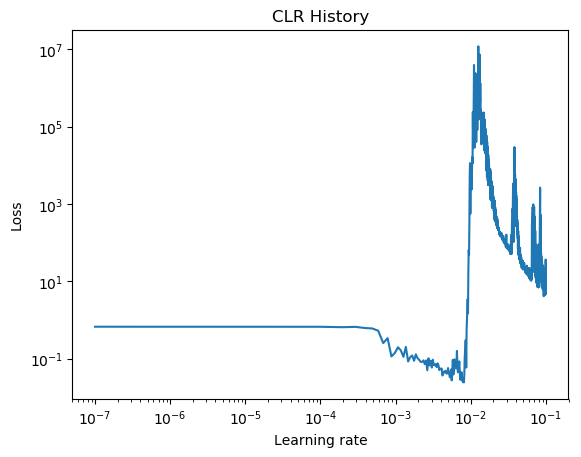
\includegraphics[width=0.49\textwidth, clip]{range_test.png}
\caption{Example output of a range test using MARGE.  For small learning rates 
(\textless 5e-4), the loss remains unchanged becaues the learning rate is too 
small to adjust the NN's weights.  Above this value, the loss begins to decrease
until around a learning rate of 8e-3, where the loss dramatically increases. 
From this range test, a good learning rate range would be perhaps 6e-4 -- 
7e-3.}  
\label{fig:rangetest}
\end{figure}

\noindent It is also important to consider the CLR mode when choosing these 
boundaries.  The `triangular' mode (which constantly varies the 
learning rate between the min/max values) allows good performance when choosing 
the min/max values from the plot, as described above.  By comparison, the 
`triangular2' mode (which performs like triangular, except that the max 
learning rate is decreased at the end of each cycle) can require users to 
select a slightly larger minimum value to achieve good performance.  This is 
because, if the minimum rate corresponds to the smallest possible change in 
loss, once the max rate has been decreased to be effectively equal to the min 
rate, it will not allow the weights to significantly change.  For this reason, 
we recommend that users select a slightly larger min value; in the example of 
Figure \ref{fig:rangetest}, a value like 7e-4 -- 9e-4 would be a good choice 
for the `triangular2' policy.  Similar precautions should be considered when 
using other CLR modes that adjust the max rate.


\section{FAQ}

This section will cover some frequently asked questions about training NNs, 
as well as specific questions about MARGE.  Have a question that isn't 
answered below?  Please send it to the corresponding author so we can add 
it to this section! \newline

\noindent \textbf{Q: I have a data set.  How should I split it into 
training/validation/testing sets?}  A: There is no set way to split the data, 
but a general guideline would be something like 70\% for training, 20\% for 
validation, and 10\% for testing.  For large data sets that contain many more 
cases than are necessary to learn the problem at hand, it may be helpful to 
reduce the proportion for training and increase the validation and/or testing 
set sizes (see next Q for related discussion).  However, we strongly advise 
against adjusting this split to improve
performance on the testing set, as that situation would mean that the testing 
set is being used for optimization rather than testing.  Users should decide 
on a split, train and validate the model, and then consider whether the split 
should be adjusted (e.g., more training cases are needed).  \newline 

\noindent Another important 
consideration is that the training, validation, and testing sets should have 
roughly equal statistical properties (mean, standard deviation, minimum, 
maximum).  This is important, as there is an implicit assumption that the 
training data statistically represents the other subsets of data.\newline

\noindent \textbf{Q: How much data do I need?} A: This is somewhat empirical, 
but in general, more data is better.  We generally advise against using small 
(\textless 10,000) data sets.  A helpful metric to consider is, if the 
parameter space were sampled on a grid, how many samples per parameter would 
your dataset result in?  For example, if I have 100,000 training cases for a 
10-parameter model, this is just over 3 samples per parameter on an 
equally-spaced grid ($3.16^{10} \sim 100000$).  For some problems, this may be 
adequate.  For comparison, consider 100,000 training cases for a 3-parameter 
model.  That would be roughly equal to 46 samples per parameter, which is 
likely more than necessary for most problems.  In that case, it would be 
advised to shift some of the training data to the validation and/or testing 
sets. \newline

\noindent \textbf{Q: How do I decide on the model architecture?} A: This is 
determined via a model grid search.  See Section \ref{sec:optarch} for 
details. \newline

\noindent \textbf{Q: How do I decide on a batch size?} A: This is largely 
selected empirically, as part of the grid search.  
Large and small batch sizes each have their own pros 
and cons, so it is generally a good idea to consider a few different sizes.  
For some problems, larger batch 
sizes can perform equivalently to smaller batch sizes yet train faster, due 
to fewer training steps per epoch.  For other problems, smaller batch sizes 
can achieve higher accuracy, as the mean squared error would be more sensitive 
to cases that perform poorly.  A good starting point is to compare the 
performance of batch sizes of 256 and 32.  Then, adjust it based on 
observations.  On GPUs, calculations will be optimized for 2\^{}N batch 
sizes.\newline

\noindent \textbf{Q: My testing set size is X, but I'm not able to plot 
the X-1 case.  Why?}  A: Because of some annoying limitations of the Tensorflow 
version used in MARGE, the data subsets are truncated to ensure an integer 
number of batches.  For example, if we have 15,000 test cases and are using a 
batch size of 256, the test set will really only have 14,848 cases (exactly 58 
batches).  A future update to MARGE's Tensorflow version may correct this 
limitation. \newline

\noindent \textbf{Q: I changed the batch size/data split/data normalization 
and now my results look horrible (e.g., negative $R^2$ values)!  What 
happened?}  A: For efficiency, MARGE 
does not produce new TFRecords or .NPY statistics files with each run; if 
they already exist, they are re-used to save compute time.  If you adjust the 
batch size, data split, or data normalization, this will adjust how the code 
works internally, but these important input files will remain unchanged, leading 
to strange behavior (e.g., negative $R^2$ values).  Whenever adjusting anything 
related to the inputs, it is advised to delete the TFRecords and .NPY statistics
files so that they are re-computed for the adjusted inputs. \newline

\noindent \textbf{Q: I'm on Mac, and I'm hitting an OMP error.  How do 
I fix this?}  A: See the Mac subsection in Section \ref{sec:install}.  Mac has 
OpenMP installed, which can conflict with some package in the conda 
environment.  The solution is to install the `nomkl' conda package.  \newline

\noindent \textbf{Q: When I try to train a model, I get an ``unable to create 
file'' error.  What's going on?}  A: The most likely cause would be that the 
filename is too long, or that the directory the weights are being saved into 
does not exist.  The latter can only happen when specifying an absolute path 
for the weight file. 


\section{Be Kind}
\label{sec:bekind}
Please cite this paper if you found this package useful for your research:

\begin{itemize}
\item Himes et al. (2020), submitted to PSJ.
\end{itemize}

\begin{verbatim}
@article{HimesEtal2020psjMARGEHOMER,
   author = {{Himes}, Michael D. and {Harrington}, Joseph and {Cobb}, Adam D. and {G{\"u}ne{\textcommabelow s} Baydin}, At{\i}l{\i}m and {Soboczenski}, Frank and
         {O'Beirne}, Molly D. and {Zorzan}, Simone and
         {Wright}, David C. and {Scheffer}, Zacchaeus and
         {Domagal-Goldman}, Shawn D. and {Arney}, Giada N.},
    title = "Accurate Machine Learning Atmospheric Retrieval via a Neural Network Surrogate Model for Radiative Transfer",
  journal = {PSJ},
     year = 2020,
    pages = {submitted to PSJ}
}
\end{verbatim}

\noindent Thanks!

% \section{Further Reading}
% \label{sec:furtherreading}

% TBD: Add papers here.


\end{document}
